
\section{Introduction}
The node-link (ball-stick) [REF SECTION] style structure has long been used to represent real-world relationships between items. Such a structure is complementary to our cognitive disposition towards pattern recognition [citep]. It is for this reason that the node-link visualisation format has been used for anything ranging from transportation maps [citep BECK] to the differentiation of ancestorial lineages of the human race (\autoref{fig:skulls}). However, the abundance and complexity of real-world data often present us with difficulties in manually representing it in a useful form. In SECTION XX it is suggested this may be overcome with the use of computational analysis and automated visualisation tools. Such methods usually require a level of data manipulation to transform the data into a machine parseable form. 

\begin{figure}[H]
     \centering
         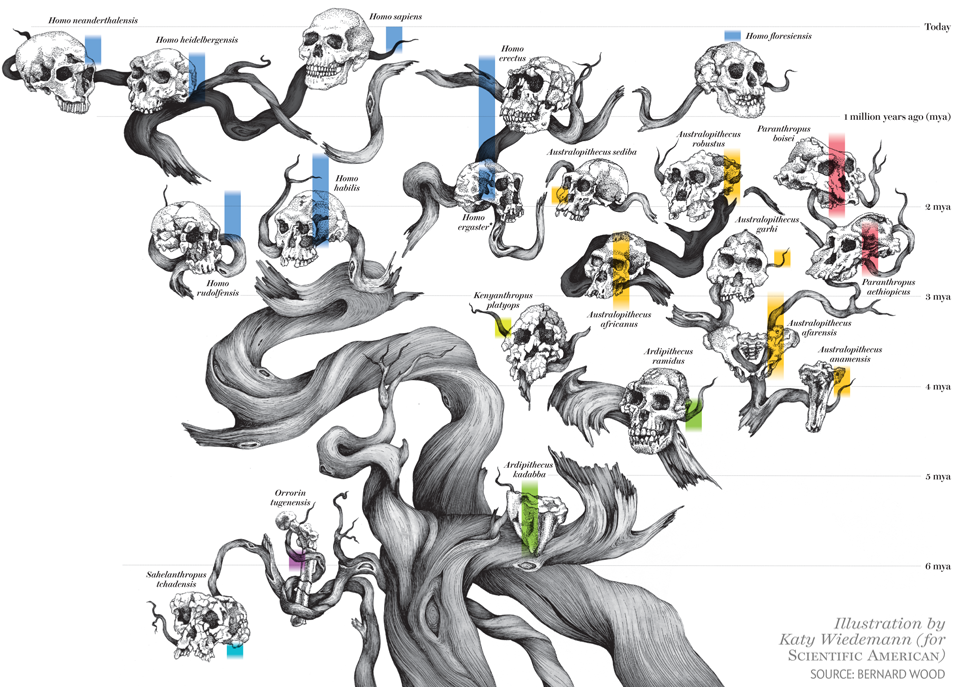
\includegraphics[width=\textwidth]{figures_c3/humanskulls.png}

        \caption[Caption for LOF]{\textbf{The human family tree.} This is a visual depiction of the human lineage, starting with our common ancestorial roots. In SECTION it was shown that the use of trees / graphs\protect\footnotemark is useful in showing relationships between items. Source: \citep{skull}}
        \label{fig:skulls}
\end{figure}
%inserted in the figure caption
\footnotetext{A tree is a special case of a graph}



In the field of mathematics a graph, $G(\nu,\epsilon,\omega)$, is defined as a function of items (vertices\footnote{The term node, item or vertex shall be used interchangeably for the remainder of this chapter. This also applies to links/relationships/edges and edge-weight/strength}), $\nu$ which are connected through a series of connections (or edges$^1$) representing any relationships between them, $\epsilon$. Since relationships in the real world are rarely equivalent, we then encode the importance of each link in the form of an edge weight, or strength - $\omega$. Such formats allow both numerical and computational algorithms to understand and interpret the graph structure, providing us with information about the data or make use of automated layout programs for visualisation. 


This chapter builds on the work shown in SECTION XXX - where 
the ability to represent complex data in the form of a graph was used to (visually) draw information regarding network structure and temporal changes. Here I will begin by exploring situations where the visual representation of many, large or complex networks is impractical. We start by introducing a series of mathematical approaches which are capable of quantifying the graph (and nodes within it) and apply them to the co-author network for papers regarding the Master Chemical Mechanism, \autoref{sec:graphmetrics}. Following these global metrics are used to categorise the chemistry within different mechanism subsets, and provide us with an insight to the chemistry structure (SECT LABEL) and finally apply these to real-world simulations representing a range of environments (marine, rainforest and urban) in SECTREF.


\textit{
This allows for a higher level of automated analysis which can be used to batch process, analyse and categorise chemical simulations. \autoref{sec:graphmetrics} begins by introducing the most common of the graph metrics which can be used for analysis. To do this a citation graph is generated by web-scraping google scholar results. 
}


\section{Graph Metrics}\label{sec:graphmetrics}

An increase in the ability to gather and store data results in a difficulty to understand it (ref SECTION). The production of large, multivariate networks of inexplicable complexity greatly hinders our ability to draw out meaningful conclusions based on visualisation alone. This means that much like the generation of mechanism, or creating semi-automated graph drawing layouts, we must rely on the field of mathematics coupled with computational aid (REF SECTION).

Numerical algorithm, derived from the field of Graph Theory can be used to circumvent the need for individual graph analysis and provide us with information about the network. One such subset of numerical algorithms are regarded as "centrality metrics", and may be used to rank the role and importance (centrality) of a node. In the following sub-section, the most common (REF PAPER) centrality metrics are discussed and applied to the MCM citation network. 


\subsection{Centrality metrics and academic publishing.}


One common application for graph analysis and visualisation is the representation and prediction of citation counts within academic journals \citep{cocite,google,naturecitation,netcoauthor}. Here network-visualisation techniques may be used to highlight the origins of a paper - for instance, \autoref{fig:naturecover} shows the multi-disciplinary research which underpins 6 prominent discoveries in the last 150 years. 

To the properties presented by different centrality metrics (described above), we apply them to an approximate representation of the citation graph relating to the Master Chemical Mechanism (\autoref{sec:metricmcm}).



\subsection{The Master Chemical Mechanism (MCM)}\label{sec:metricmcm}

The MCM, \citep{mcm}, is a near explicit representation of our foremost understanding of gas-phase tropospheric chemistry. The mechanism describes the oxidation of 143 primary emitted VOCs and the respective rates at which this occurs. It has been used in the... 



 Information on the chemistry, - x species - y ... first published and how this can be used with regards to the following algorithms are presented in REF JENKINS 15 ACP. 


\begin{figure}[H]
     \centering
         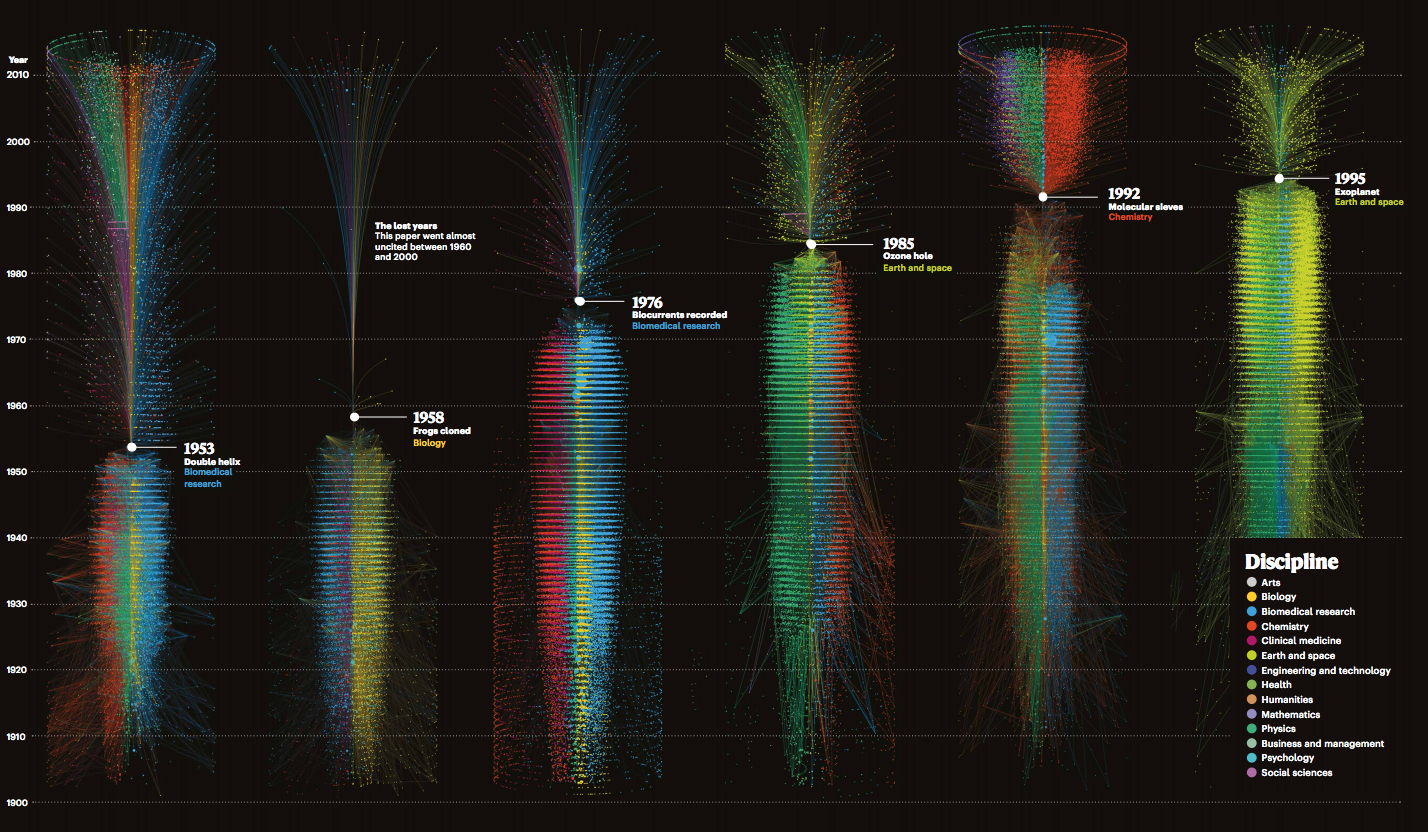
\includegraphics[width=0.92\textheight,angle=90]{figures_c3/naturegraph.png}

        \caption{\textbf{150 years of letters to Nature.} A visualisation showing how previous research is used to inspire future studies. Important discoveries (DNA, Cloning(frogs), Bio-Currents, Ozone Hole, Molecular Sieves and Exoplanets) are split into research which contributed to their formation (below), and the consequent papers produced from each discovery. Use of colour is used to emphasise the multi-disciplinary nature of prolific scientific discovery. Source: \citep{naturecover}}
        \label{fig:naturecover}
\end{figure}



\subsection{Data Collection}\label{sec:scholar}

To generate a dataset on papers related to the MCM. The academic search engine (Google Scholar \citep{scholar}) is queried for all articles containing the words \{ \emph{"Master", "Chemical", "Mechanism"} and \emph{"MCM"} \}. For each match, the first 100 pages of results are selected. Each of these contains 10 articles, from which the first 100 pages of related articles are chosen.
In taking the top 1000 citations for each page a network of 15744 papers and 30178 citations\footnote{Note: this had the potential of returning up to 1000,000 nodes} is created. This process made use of an edited version of the  \emph{etudier} Github repository, \citep{web}.


\subsection{Visualising the data.}

The initial visualisation of the dataset is accomplished through the use of THREE.js \citep{threejs}. This makes use of WebGL bindings and allows for the efficient viewing, querying and interacting of the data in 3 dimensions. This helped identify the temporal changes within the network by mapping a papers publication year to the $z$ direction, \autoref{fig:weball}, as discussed in \autoref{sec:filter3d}. 

\begin{figure}[H] %dont leave blank lines between sfig
     \centering
     \hfill
     \begin{subfigure}{0.495\textwidth}
         \centering
         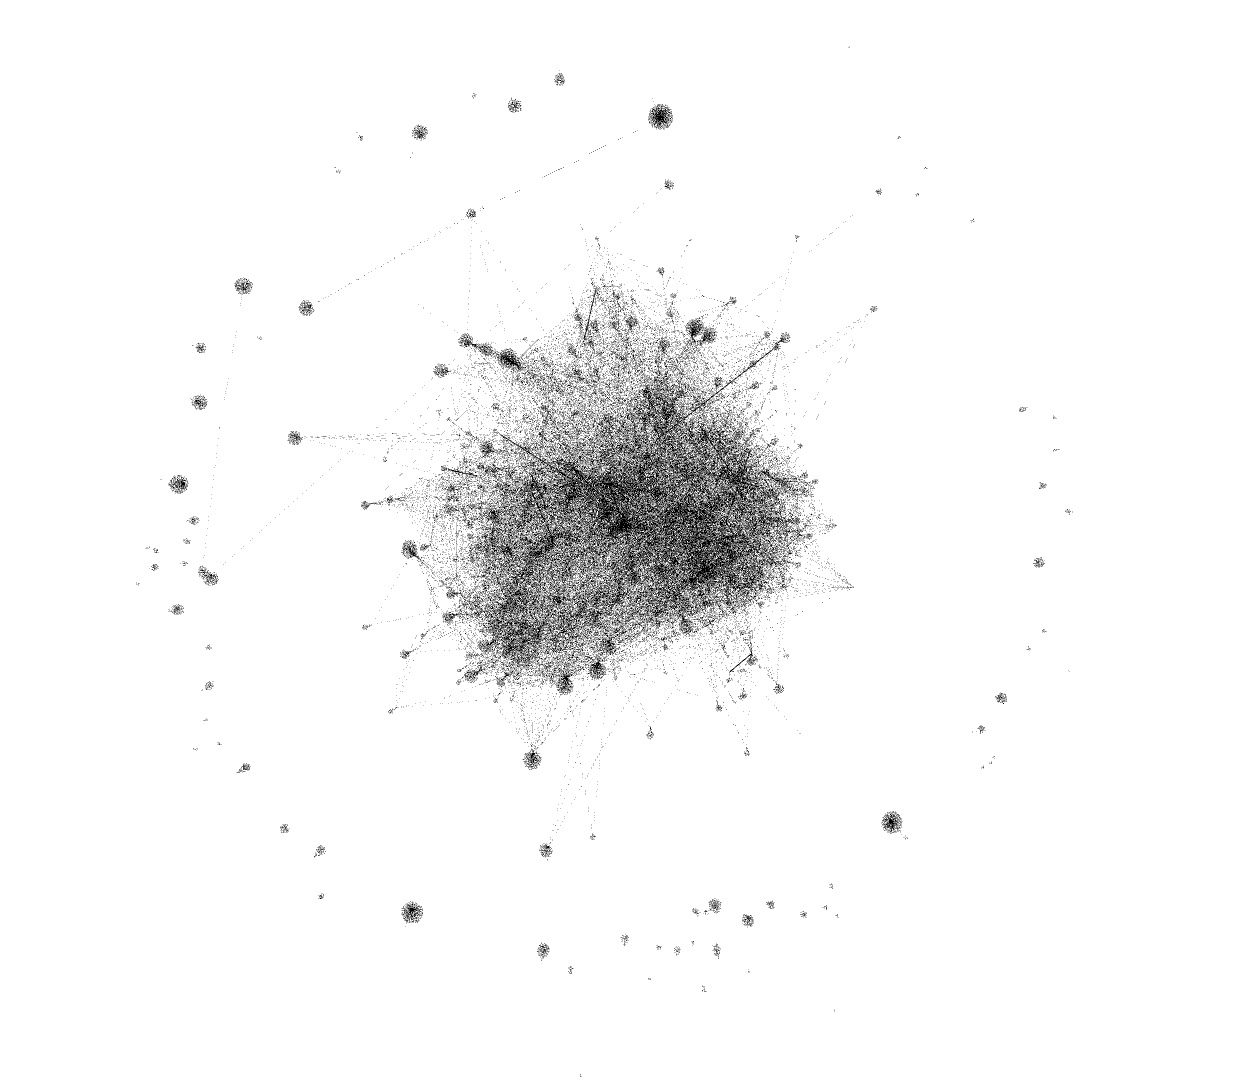
\includegraphics[width=\textwidth]{figures_c3/gephiall.png}
         \caption{A 2D force directed representation of the network using the gephi software \citep{gephi}}
         \label{fig:gall}
     \end{subfigure}
     \hfill
     \begin{subfigure}{0.47\textwidth}
         \centering
         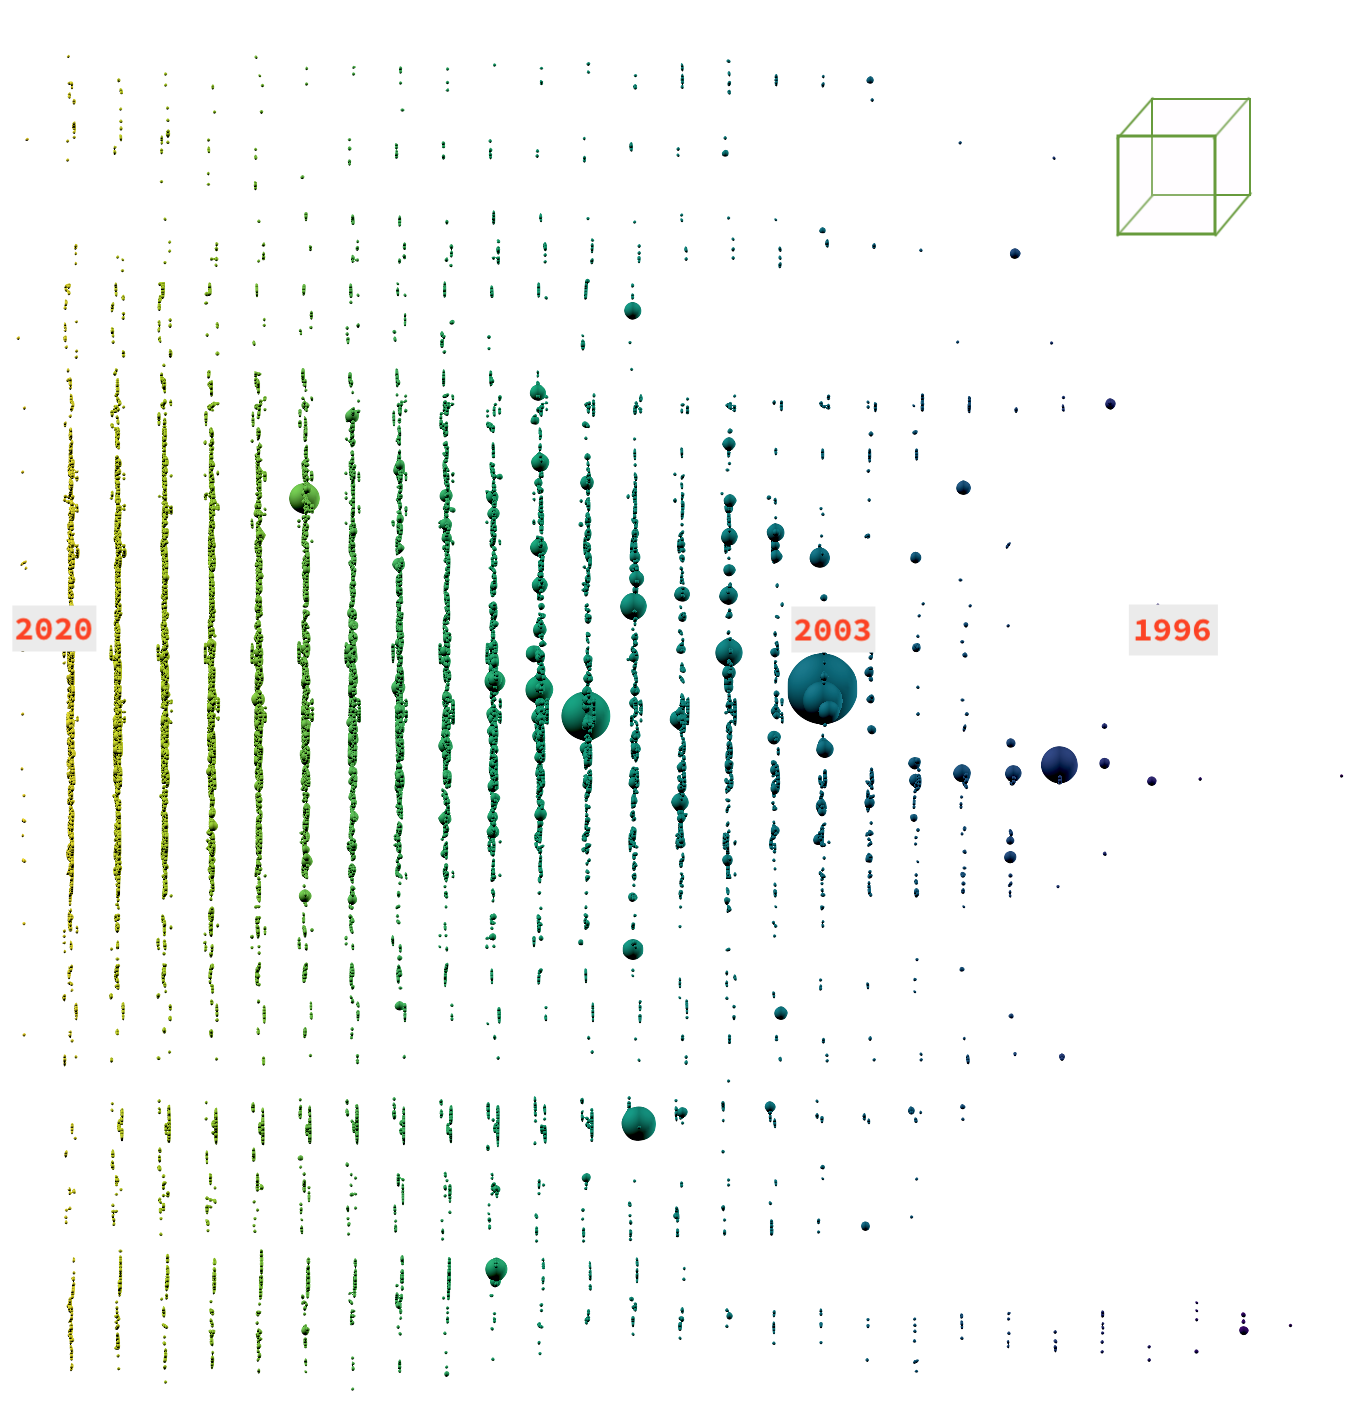
\includegraphics[width=\textwidth]{figures_c3/sideall.png}
         \caption{3D orthographic camera (sideview)}
         \label{fig:sideweb}
     \end{subfigure}
     \hfill

     \begin{subfigure}[b]{0.75\textwidth}
         \centering
         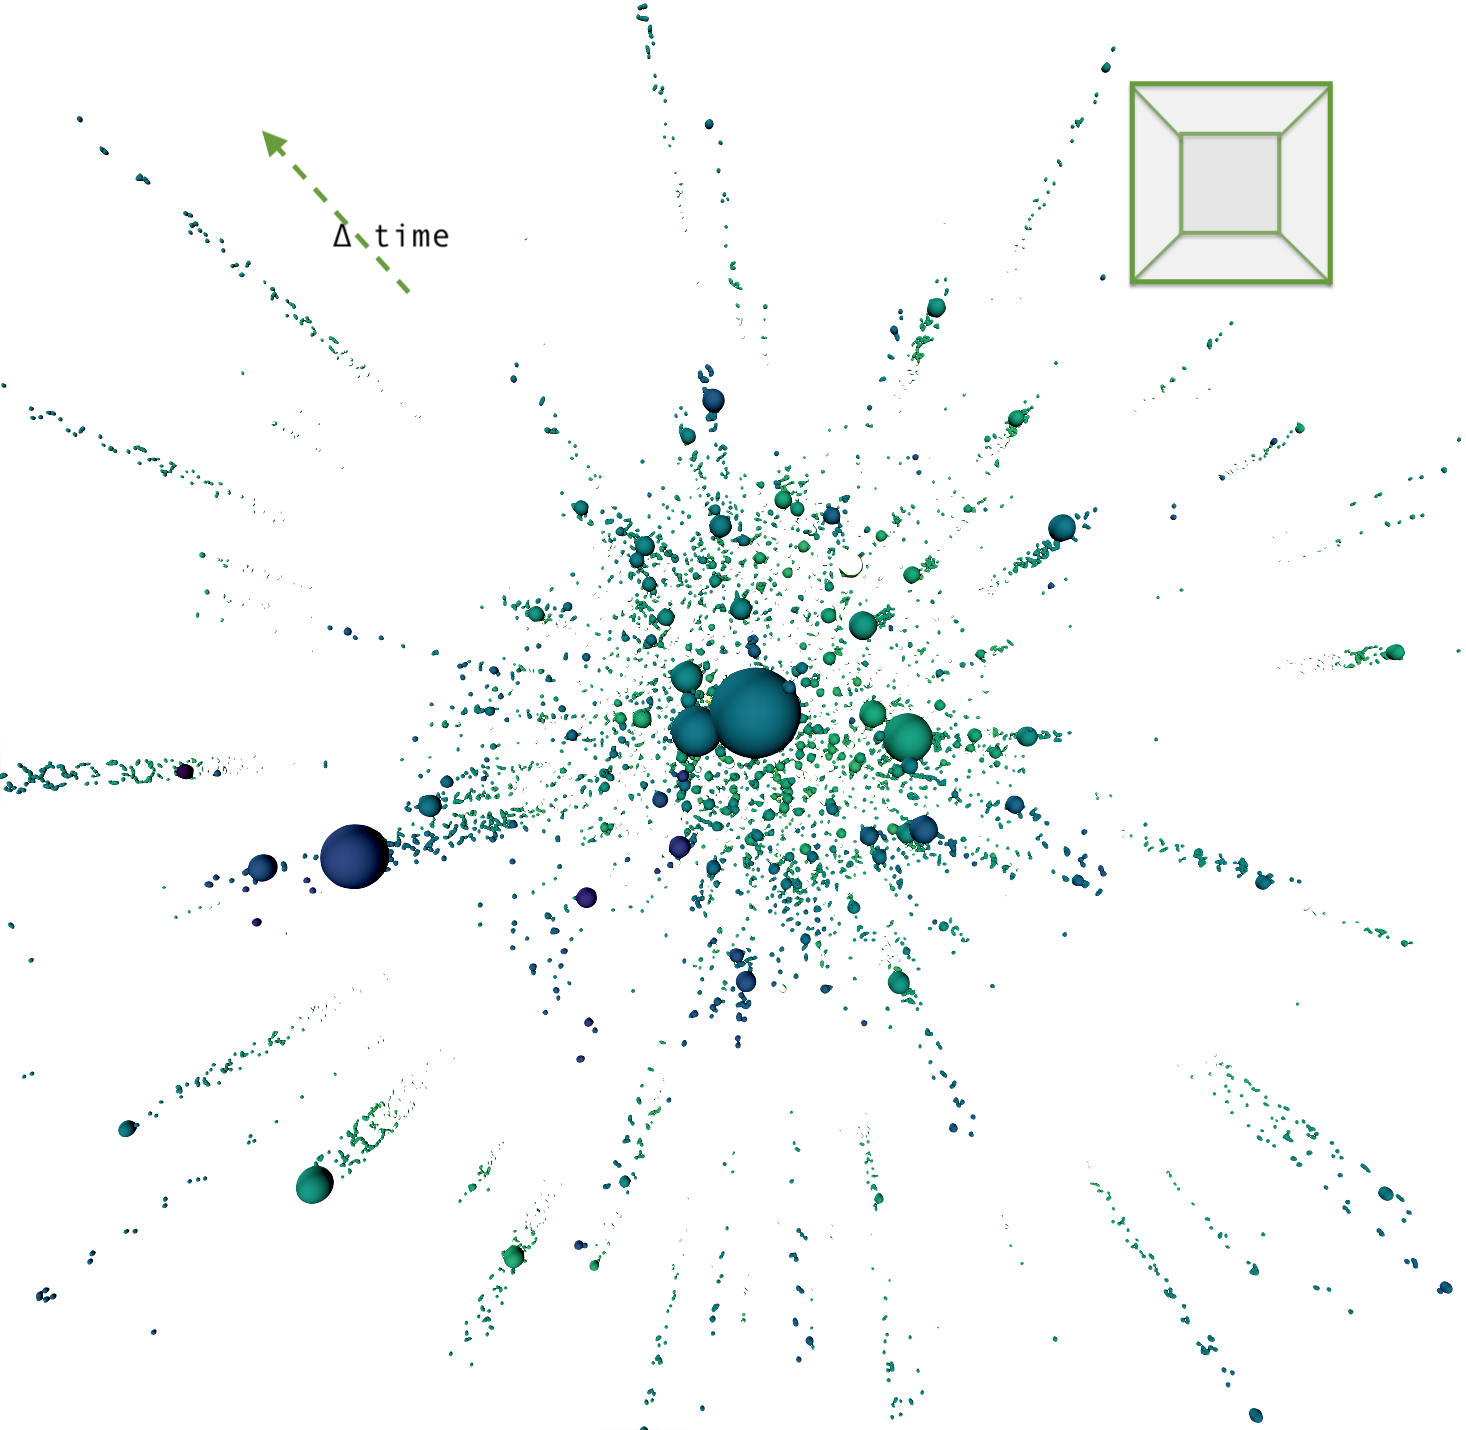
\includegraphics[width=\textwidth]{figures_c3/threeall.png}
         \caption{3D perspective camera}
         \label{fig:3dgeph}
     \end{subfigure}


        \caption{ \textbf{Initial 3D graph representation of the scraped MCM citation graph.} (a) shows the `classic' graph representation of the network. (b) shows a size representation using an orthographic perspective. Here time is shown across the $x$ axis, with yellow being the most recent. (c)
        uses a perspective camera, which emphasizes the...
        Still captures of 2D and 3D visualisations of the dataset. Node size corresponds to the number of citations, and colour (and z-axis) corresponds to the publication year for each paper.}
        \label{fig:weball}

\end{figure}


\subsection{Filtering the data}\label{sec:filter3d}


In the method used to web scrape data, there are several features which need to be corrected/removed. The reasons for this are discussed below.
 
\paragraph*{Pre-1996}
There exist several papers predating the conception of the MCM (1996). A number of these can be attributed as incorrect data, with publication dates <1900 which may be the result of missing information or a fault in googles web scraping algorithm. Any such papers are removed from the dataset.

 For otherwise correct articles, those published pre-1996 are also filtered from the dataset - this is because we are interested in identifying the influence the MCM has had on research and not the research that may have led to its creation. This can be seen in the cone-like shape emanating from the first MCM papers in \autoref{fig:sideweb}.

\paragraph*{N-th degree research}
Not all research articles in a field reference other articles with the same field. \autoref{fig:naturecover} showed us that many of the great discoveries in science have a multidisciplinary nature. It is for this reason that it is expected that articles from non-atmospheric areas of research may reference or build upon specific areas of research touched by the MCM. Such papers, and in consequence the papers which cite them, have little or no links to many of the core MCM papers. Such papers manifest themselves as a halo of satellite clusters which are connected by themselves but not with the main body of the graph, \autoref{fig:gall}. In using a 3D perspective viewpoint (\autoref{fig:3dgeph}) it is possible to identify the paper which references the MCM and then the consequent papers which cite it by observing the satellite clusters, and the gradually lightening spiral of papers which emanate out of it. 

Analysis of the network connections for each cluster can allow us to identify the indirect relationships some of these diverse topics (\autoref{table:otherpapers}) contained within the satellite nodes. Here it can be seen that the use of photochemical ozone creation potentials \citep{milk1,milk2} are used for the Life cycle assessment of Italian high-quality milk production \citep{milk}. 
Similarly indirect paths such as the paper:
 "Temporal controls on dissolved organic matter and lignin biogeochemistry in a pristine tropical river" (\citep{biogeo}) can be used to link to \citep{georiver1} and ultimately the MCM protocol paper \citep{mcmpartA}.
 
 If we desired to remove such papers, the simplest method would be to recreate the graph into one where links are drawn between papers that are cited together (\autoref{sec:cocitep})
 and then removing any nodes without any external connections (isolates).

\begin{table}[H]
\begin{center}
\begin{tabular}{ p{0.6\textwidth}|l }
 \hline
   & \\
 Fabrication of Bioinspired Actuated Nanostructures with Arbitrary Geometry and Stiffness & \citep{nano} \\ \\
 %
 Temporal controls on dissolved organic matter and lignin biogeochemistry in a pristine tropical river  & \citep{biogeo} \\ \\
Neuroproteomics in Neurotrauma & \citep{neurotrauma}\\ \\
%
Fast start-up of a pilot-scale deammonification sequencing batch reactor from an activated sludge inoculum & \citep{pilot} \\ \\
Red blood cell oxidative stress impairs oxygen  delivery and induces red blood cell aging & \citep{blood} \\ \\
%
Life cycle assessment of Italian high quality milk production. & \citep{milk}\\ \\
%
 \hline
\end{tabular}
\end{center}

\caption{A selection of research papers not directly connected to the field of atmospheric modelling.}
\label{table:otherpapers}
\end{table}



\paragraph*{Unprobable occurances}
Finally, the extracted network also contains many disconnected component subgraphs - graphs with no connection to atmospheric science. An example of this is seen in an article about neuroproteomics in neurotrauma \citep{neurotrauma}. In analysing the paths which connect this, it is seen to cite the paper on "Large scale gene expression profiling of metabolic shift of mammalian cells in culture", \citep{neuro2}. This is an anomaly which within its structure contains the words "Master", "Chemical" and "Mechanism" (separately) and has `MCM' as an abbreviation for one of the author names. To remove such papers, all disconnected sub-components are removed from the analysis. 



\paragraph*{A note on unintentional filtering}

\textit{
Author names and some extended titles may be truncated with the use of ellipses. This is due to the web scraping script extracting these directly from the Google scholar page, and not the original articles themselves. It is worth noting that the results in this section are not explicit, but rather a demonstration of graph theory on a real-world dataset.
}


\subsection{The Co-citation Network}\label{sec:cocitep}

The document coupling techniques of co-citation was introduced in the 1970s as an alternative approach for quantifying the results within the science citation index \citep{cocite}. Rather than representing a graph using backpropagation (through the use of referencing and citation counts), a co-citation network introduces a link between papers if, and only if, they have been cited together. Although this loses the directionality of a graph, it allows us to show forward propagating trends between papers within the same field. 

Applying the above method allows us to reduce the citation graph of 451 papers and 5402 edges to an undirected co-citation graph of 2758 edges - halving the number of original links between papers. 

\subsection{The Co-authorship network}
An alternative to exploring which papers which are cited together are to look at their authors. Here undirected links are drawn between authors on the same paper. This style of analysis was used to show that the number of papers per author, and the total number of authors per paper can vary between research fields, \citep{newmancoauthor}. In combining this with a series of network centrality metrics, \citep{coauthornew} revealed that it is possible to discern promising researchers from both iter and Intra disciplinary groups. 

In building a co-authorship network for the MCM, we can identify authors who publish together\footnote{ Disclaimer: as mentioned earlier, not all authors for every paper were recorded by the web scraping algorithm} and highlight research groups who work with the MCM, \autoref{fig:authorgroup}. This shows how authors with a similar geographic location/institution are more likely to publish together. The largest cluster here falls under the MCM developer team, which resides between the Leeds and York universities. Next two German institutions which are heavily involved in the atmospheric chemistry field (Julrich and Max Planck), followed by an assortment of Chinese authors, mainly centred around the Beijing or Hong Kong region. 


\begin{figure}[H]
     \centering
         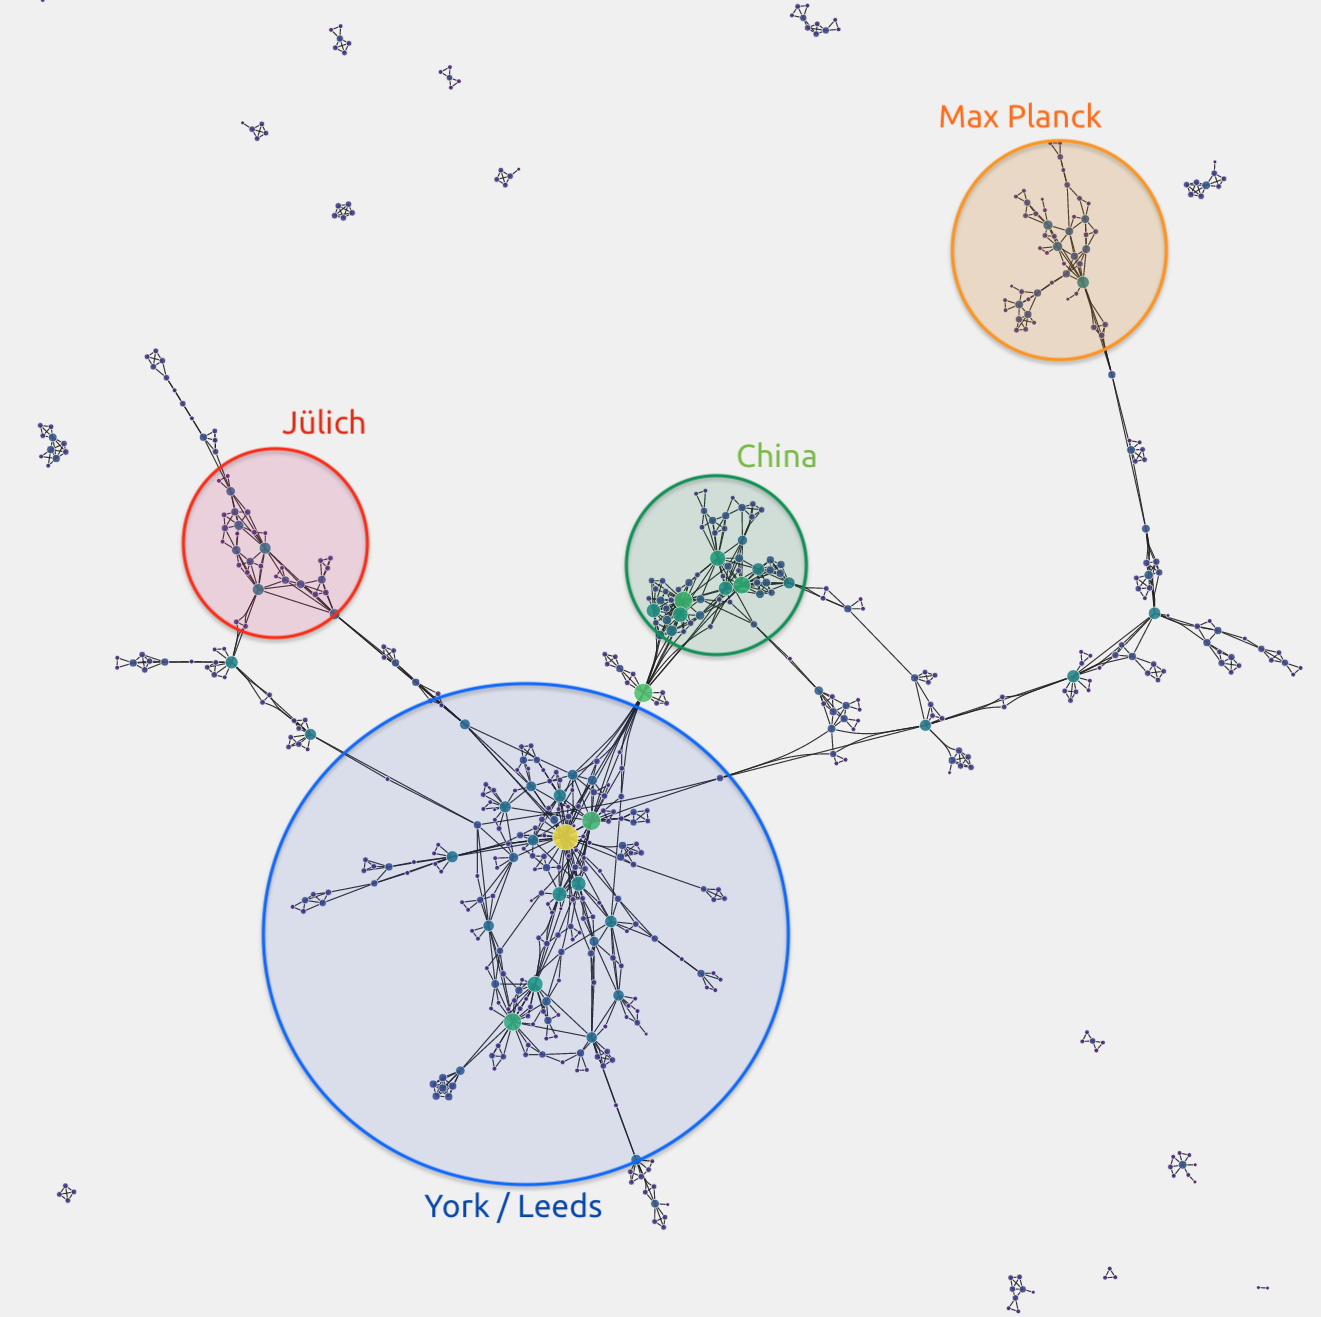
\includegraphics[width=.8\textwidth]{figures_c3/GroupAuthor.png}
        \caption{ \textbf{The co-author network.} In representing the authorship network as a force directed graph we are able to see cliques or clusters of people who publish together. It can be noted that this often occurs when they have a similar geographical location.}
        \label{fig:authorgroup}
\end{figure}


